%# -*- coding:utf-8 -*-

\section{研究现状}
\label{sec1-3}

%本节叙述内容:
%\begin{enumerate}
%  \item 国外研究现状
%  \item 国内研究现状
%  \item 相关技术现状
%\end{enumerate}

在军事和工业领域,基于虚拟现实的仿真技术在训练、以及评估在特定环境下使用者解决问题的反应等方面,已经显示了重大的实际价值 \cite{Goodwin1978Simulator,Rolfe1986Simulators,Ressler1999Simulators,Wachtel1985Simulators,Liu2013Military}。%
经过数十年时间的发展 \cite{Dawson1998},仿真技术在医学、尤其是医学训练领域的应用也已经比较广泛,包括内窥镜 \cite{Vining1995Endoscopy,Preminger1996Endoscopy}、神经医学\cite{Kockro2000Neurosurgery,Cotin2005EVE,Ma2007NeuroCath}、麻醉学\cite{Gaba1988Anesthesiology}、支气管镜\cite{Vining1996Bronchoscopy}、腹腔镜\cite{Hon1994Laparoscopy,Derossis1998Laparoscopy}、以及心血管和外周血管系统的介入手术\cite{Chui1998ICard,Cotin2000ICTS,Tan2012NUDT}等。%
2004年,美国食品药品监督管理局(FDA)决定,行颈部血管介入手术等高风险手术的医生,必须在术前进行技能训练,直到精通为止,而且对这种技能的初期训练实践不能在病人身上进行 \cite{Dawson2006Medicine}。%

受经济、文化、公共卫生管理、医学和工程技术等诸多因素的制约,我国在这方面的研究和应用与欧美发达国家相比,尚有不小差距,具体表现在研究水平和应用水平等两方面。
本节将分别介绍国内外科研人员在虚拟医学训练、尤其是血管介入术虚拟训练以及相关研究方向上所作的主要工作和重要成果。

\subsection{国外研究现状}
\label{sec1-4-1}

最早出现的介入放射学仿真系统之一是美国HT Medical公司开发的Dawson-Kaufman血管介入放射学虚拟系统 \cite{Higgins1995DK,Dawson1996DK,meglan1996DK}。
该系统首先用于腹主动脉介入的仿真 \cite{Wang1998ICard}。
系统所提供的解剖环境基于真实病例的影像,并在此基础上重建了血管的静态刚性模型,整个解剖环境模型被渲染成与术中X光影像类似的显示效果以提高仿真的真实性 \cite{Higgins1995DK}。
同时,该系统还能够通过专门设计的触觉接口装置为使用者提供“真实”的导丝操作感受 \cite{BroNielsen1997DK}。
通过这些技术,Dawson-Kaufman介入放射学虚拟系统为使用者提供了实践血管成形术和其它疏通阻塞血管的技术的训练平台。

同期出现的还有新加坡国立大学和美国约翰·霍普金斯大学医学院共同研究与实现的用于腹部主动脉介入仿真训练的daVinci系统(\textbf{\textit{Vi}}sual \textbf{\textit{n}}avigation of \textbf{\textit{c}}atheter \textbf{\textit{i}}nsertion \cite{Lawton2000daVinci}) \cite{Anderson1996daVinci,Anderson1996adaVinci,Anderson1997daVinci,Anderson1997adaVinci}。%
该系统利用了美国“可视人计划”(\textbf{\textit{V}}isible \textbf{\textit{H}}uman \textbf{\textit{P}}roject, VHP) \cite{vhpweb}的人体数据,通过与X光效果的解剖背景配准的仿真血管模型,向使用者提供实时的平面可视效果以及立体的导管导航\cite{Anderson1998daVinci}(见图\ref{fig1-1})。%
血管壁由包围血管壁的内部区域的势能场来表示,这个势能场决定了导管和血管壁之间相互作用的能量,导管的建模采用有限元方法,把导管抽象为六自由度的梁元 \cite{Chui1996daVinci,Wang1996daVinci}。%
虚拟导管的材料特性通过杨氏模量和切变模量来体现,但忽略了导管与血管壁之间的摩擦力 \cite{Anderson1998daVinci}。
Lawton等人 \cite{Lawton2000daVinci}还开发了一种物理模型和数值算法,用于仿真将导管插入动脉系统并推进的过程。

%\begin{figure}[!ht]
%\centering
%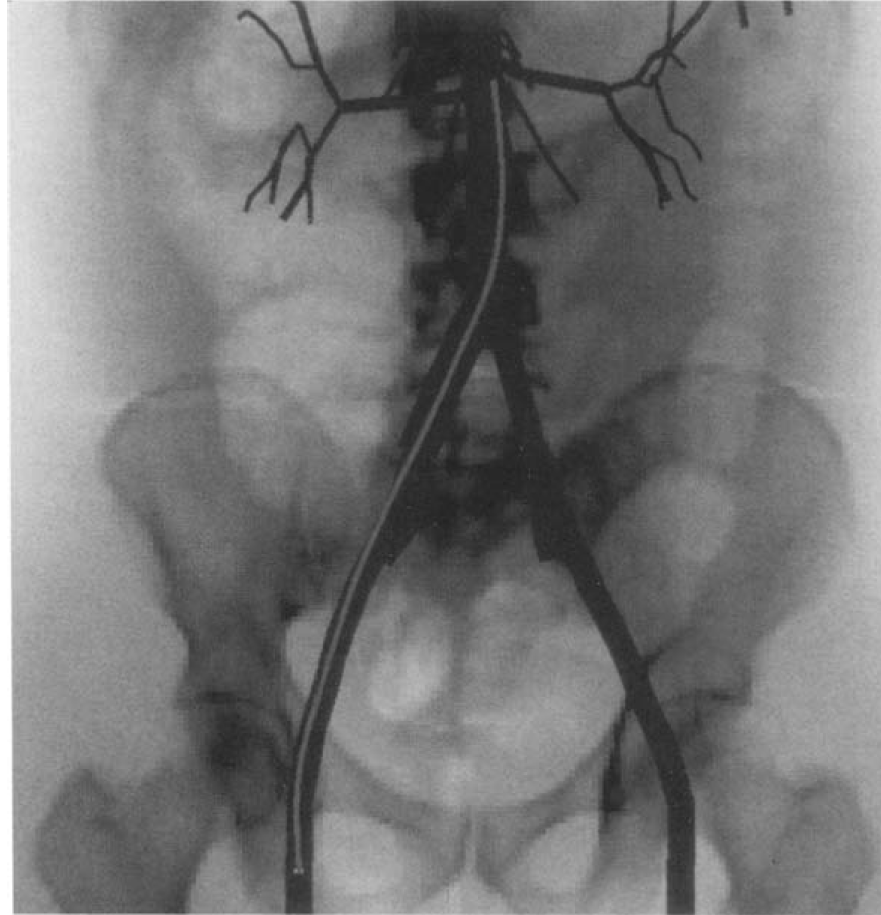
\includegraphics[scale=0.5]{Figures/DaVinci.png}
%\caption{新加坡国立大学和美国约翰·霍普金斯大学医学院共同研究的腹主动脉介入仿真训练系统daVinci\cite{Anderson1998daVinci}}
%\captionof{figure}[腹主动脉介入仿真训练系统daVinci]{新加坡国立大学和美国约翰·霍普金斯大学医学院共同研究的腹主动脉介入仿真训练系统daVinci\cite{Anderson1998daVinci}}
%\label{fig1-1}
%\end{figure}

几乎与此同时,开发daVinci的科研团队在前期工作的基础上,先后实现了用于心血管介入仿真训练的ICard系统(\textbf{\textit{I}}nterventional \textbf{\textit{Card}}iology Simulator) \cite{Wang1997ICard,Chui1998ICard,Wang1998ICard,Cai2004ICard,Cai2006ICard},以及用于脑血管介入仿真训练的NeuroCath系统(\textbf{\textit{Neuro}}radiology \textbf{\textit{Cath}}erization Simulator) \cite{Ma2000NeuroCath,Nowinski2000NeuroCath,Ma2001NeuroCath,Li2001NeuroCath,Nowinski2001NeuroCath,Anderson2001NeuroCath,Chui2002NeuroCath,Anderson2002NeuroCath,Ma2004NeuroCath,Volkau2005Vessel,Ma2005NeuroCath,Ma2006NeuroCath,Ma2006aNeuroCath,Ma2007NeuroCath}。%

ICard系统的应用目的是为医学院学生和医生提供一个能够方便地温习心血管介入疗法的平台,同时还希望兼顾评价使用者的技能水平。
该系统的软件部分提供了血管的立体模型和X光效果的显示 \cite{Wang1998ICard,Wang1998aICard}。
血管的影像数据主要来源于VHP。
对于手术涉及的主干血管,限于当时计算机的处理能力,研究团队使用Adobe Systems公司的Photoshop从每张横切影像中将感兴趣的区域中的血管影像的围线标出,然后再计算血管的中心线,最后结合中心线上各点的坐标和相应的半径,得到血管的模型 \cite{Wang1998ICard}。%
对于病灶涉及的冠状动脉,由于尸体的血管内并没有血液流动以及因此产生的压力,因此这部分较细的血管就会因为其周围肌肉组织的挤压而导致严重变形,这也就造成VHP数据中,冠状动脉的数据几乎全部被破坏 \cite{Wang1998ICard}。%
为了解决这个问题,该团队的研究人员利用三次元量床(\textbf{\textit{C}}oordinate \textbf{\textit{M}}easuring \textbf{\textit{M}}achine,CMM)\cite{CMMweb}来扫描冠状动脉的钢质模型 \cite{KyotoModelweb},从而获得包括完整冠状动脉分支的仿真血管网络,再经过后期的细部处理,得到满足系统要求的冠状动脉血管模型 \cite{Wang1998ICard}。%
此外,ICard系统还提供了人体的脑血管模型 \cite{Serra1997Vessel,Poston1995Vessel},而脑部影像数据是一组核磁共振血管影像 \cite{Wang1998ICard}。
然后,他们通过配准将上述的心脑血管模型与VHP中的主干血管模型连接在VHP数据构建的解剖环境中来获得完整的血管模型 \cite{Wang1998ICard}。
至于导管的建模,该系统同样采用了有限元方法 \cite{Wang1998ICard}。
ICard提供了两种不同的交互方式:一种是计算机界面,另一种是物理装置界面 \cite{Wang1998ICard}。
前者通过点击图形界面上的按钮;后者则通过专门设计的物理装置(导管移动传感装置,\textbf{\textit{C}}atheter \textbf{\textit{M}}ovement \textbf{\textit{S}}ensor device, CMS) \cite{Lim1998ICard,Lim1997ICard}。%
ICard的软件系统所支持的功能包括X光影像显示、立体影像显示与横切面显示、生物医学信号模拟、球囊与支架的植入、以及诸如造影剂的注射等 \cite{Wang1998ICard}。

NeuroCath用于仿真球囊和支架的安置、动脉瘤弹簧圈栓塞术(Aneurysm Coiling)等脑血管介入手术。
它继承了前两个系统的许多成熟技术和特性,包括:基于有限元方法的导丝建模以及导丝与血管壁相互作用建模 \cite{Wang1996daVinci,Chui1996daVinci}、基于多模态影像的血管中心线提取 \cite{Wang1998ICard}、以及X光效果的显示\cite{Wang1998aICard,Wang1998ICard}等。%
在此基础上,该系统为使用者提供了尽可能丰富和接近真实的体验。如:造影剂注入后在血管内扩散现象、虚拟病人在虚拟手术过程中的生理表征等。
为获得NeuroCath系统所需的脑血管模型,Cai等人 \cite{Ye2002Vessel,Cai2003aVessel,Cai2003Vessel}采用了一种利用扫描和混合操作以生成血管段和分岔的结构性方法,该方法提高了血管分岔处的光滑度;Volkau等人 \cite{Volkau2005Vessel,Volkau2008Vessel}在此基础上提出了基于血管中心线的重建方法,该方法首先提高了血管中心线的光滑程度;其次抑制了在分割和骨架化过程中引入的噪声,从而提高了(重建血管时所依赖的)血管半径的精确度。%
NeuroCath的操作风格与ICard类似,也提供了可视界面交互和物理交互装置交互两种方式 \cite{Nowinski2001NeuroCath}。
其中,研究人员为NeuroCath专门设计了物理交互装置 --- TiC(\textbf{\textit{T}}actile and \textbf{\textit{i}}mage \textbf{\textit{C}}ontrol)\cite{Chui1999TiC} \cite{Ma1999TiC},它由触觉子系统和影像操作子系统等两个主要部分组成。%
前者可以使操作者能够操作导管和导丝进行与真实血管介入手术中类似的运动;后者则通过一台虚拟工作站来操作可视界面中提供的X光影像的视角。
此外,NeuroCath还能为使用者提供血管内的视角,该功能用于血管内窥镜导航的仿真 \cite{Nowinski2001NeuroCath}。
NeuroCath最初在约翰-霍普金斯大学医学院进行了验证,随后还获得了包括德国萨尔大学诊断介入神经放射学诊所、中国北京宣武医院、以及德国国立信息技术研究中心等医院和研究机构的验证许可,并收到了比较满意的反馈 \cite{Ma2007NeuroCath}。%

为了提高工作效率,科研团队还开发了若干CAD软件,它们分别用于导管等血管介入器械,如:CathWorks \cite{Cai1998CathWorks,Cai2000CathWorks}、DCSM \cite{Li2001DCSM}等;以及血管等人体器官的建模的CAD软件工具,如:VasWorks \cite{Cai2003Vessel}、Vascular Editor \cite{Ma2007NeuroCath}等。%

近几年,该团队仍有部分研究人员致力于心血管介入手术仿真的研究,重点是心脏建模 \cite{Chiang2011,Chiang2012}等。

位于美国麻省的三菱电气实验室(Mitsubishi Electric Research Laboratories,MERL) \cite{merlweb}和美国创新微创疗法中心(Center for Innovative Minimally Invasive Therapy,CIMIT) \cite{cimitweb}联合发起了ICTS项目 \cite{Dawson2000ICTS,Cotin2000ICTS,Shaffer1999ICTS}。%
ICTS的全称是“Interventional Cardiology Training System”(介入心脏病学训练系统),该系统旨在为学习者提供训练平台,并为引入新的医学器材和手术方法提供展示平台 \cite{Cotin2000ICTS}。%
ICTS实现了X光效果的解剖环境、建立了导管的物理模型和血液流动模型、并制作了触觉接口装置 \cite{Cotin2000ICTS}。%
此外,该系统还实现了一种手术学习机制“Virtual Rounds” \cite{Shaffer1999ICTS},该学习机制复现了心血管介入手术的基本步骤,为使用者的训练评估提供了基础。
文献 \cite{Dawson2000ICTS}中提到,ICTS系统当时正准备在欧洲投入其首次训练试验。

然而,当时的ICTS仅仅处于样机验证阶段,根据与比利时Guidant公司的合同,该项目后来被移交至英国Virtual Presence公司以完成系统的研发,并最终由瑞典Mentce公司 \cite{menticeweb}将其商业化 \cite{GuidantMenticeNewsWeb,coles2011surveyCRaIVE},这就是该公司的VIST系列产品。%
目前,VIST系列的两种仿真平台已经能够仿真的血管介入技术有:冠状动脉造影、心脏节律管理、跨室间隔穿刺、肾动脉介入、髂内动脉介入、膝关节以下血管介入、主动脉内窥修复、颈动脉介入、脑血管介入、子宫动脉栓塞术等 \cite{menticeweb}。%
其中已经获得医学验证的技术有:颈动脉介入手术的仿真训练 \cite{Dayal2004VIST,Hsu2004VIST,Nicholson2006VIST,Patel2006VIST,Cates2007VIST,VanHerzeele2009VIST},肾动脉介入术 \cite{Aggarwal2006,Glaiberman2008VIST},髂内动脉介入术 \cite{Chaer2006VIST,Berry2007VIST,VanHerzeele2008VIST},冠状动脉介入术 \cite{Gallagher2006VIST}等。%

CIMIT的Sim小组 \cite{medicalsimweb}和法国INRIA的Shacra团队 \cite{shacraweb}联合开发的EVE项目 \cite{Wu2005EVE}是一种用于仿真脑血管介入手术的系统。
它提供了适用于复杂血管系统内部的具有实时的碰撞检测和碰撞响应性能的导管有限元模型 \cite{dequidt2007EVE,Duriez2006EVE,Lenoir2006EVE,Lenoir2005EVE,Cotin2005EVE},具有X光显示效果的头颈部解剖模型 \cite{Wu2011EVE,Luboz2005EVE,Muniyandi2003EVE},以及血流动力学模型、虚拟造影剂、心脏搏动和呼吸 \cite{Wu2007EVE}等视觉效果。%
文献 \cite{Dequidt2008EVE}介绍了该团队进行动脉栓塞术中弹簧圈的仿真以及验证的情况。
操作装置方面,研究人员设计了专用的触觉接口装置ABEL和专用的径向跟踪装置Cain \cite{medicalsimweb}。

此外,Shacra团队在EVE等项目的工作基础上,开发并维护着一个专门用于医学仿真的工具库 --- SOFA(\textbf{\textit{S}}imulation \textbf{\textit{O}}pen \textbf{\textit{F}}ramework \textbf{\textit{A}}rchitecture) \cite{Allard2007SOFA}。%

意大利CRS4小组发起了ViVa项目(\textbf{\textit{Vi}}rtual \textbf{\textit{Va}}scular project) \cite{abdoulaev1998},该项目的研究目标是为现代血流动力学研究者和心脏内科医生提供一系列的工具,帮助他们分析和解释在研究和临床过程中遇到的不断增多的相关信息。%
这些工具包括:图像处理与分割、实时立体体数据可视化、立体几何重建、立体网格生成、以及血流仿真和可视化等。
在此基础上,Gobbetti等人 \cite{Gobbetti1998}研究并实现了用于仿真血管镜的系统。
该系统以从标准医学影像模态所获取的数据作为输入,将其当作可供交互的虚拟环境;系统支持立体直接体绘制的实时导航和动态内窥镜的控制,可交互的组织分类,以及为实现形态学特性测量而摘取可交互点等。
Zorcolo与Gobbetti等人 \cite{Zorcolo1999,Gobbetti2000,Zorcolo2000}开发了一种实验性的导管插入系统。
该系统支持头部跟踪的立体视感,该视感通过从不同视角观察体重建而产生,体重建则与直接的立体触觉交互相匹配,这属于增强现实系统的范畴。

英国的CRaIVE(\textbf{\textit{C}}ollaborators in \textbf{\textit{R}}adiological \textbf{\textit{I}}nterventional \textbf{\textit{V}}irtual \textbf{\textit{E}}nvironments) \cite{CRaIVEweb}进行了与介入手术的仿真训练相关的研究。%
他们的研究主要集中于血管介入手术中血管系统的分割与重建 \cite{Luboz2008aCRaIVE},血管和导管及其相互作用的建模和验证\cite{Luboz2010CRaIVE,Luboz2009aCRaIVE,Luboz2008CRaIVE},Seldinger穿刺术的仿真\cite{luboz2009CRaIVE,John2008CRaIVE},以及穿刺术之前的腹股沟触诊的仿真\cite{Coles2011CRaIVE,Coles2009CRaIVE}。%
此外,文献 \cite{Coles2010CRaIVE}还对若干应用于穿刺仿真中的触觉反馈装置的性能进行了测试和比较。

法国巴黎第十二大学计算机工程与自动化实验室进行了基于虚拟现实技术的腹主动脉介入手术仿真系统的研究 \cite{Ghembaza2004Paris12U}。
系统中,腹主动脉和导管的物理模型采用基于位移的有限元方法来建立;为了实现连续的碰撞响应,研究人员采用了基于Cubic Spline的参数估计方法。

由荷兰列文胡克癌症研究所和乌德勒支大学图像科学研究所发起的MIVIS项目(\textbf{\textit{M}}inimally-\textbf{\textit{I}}nvasive \textbf{\textit{V}}ascular \textbf{\textit{I}}ntervention \textbf{\textit{S}}imulation) \cite{alderliesten2002NKI,Konings2003NKI,alderliesten2004NKI,Bosman2005NKI,alderliesten2007NKI,alderliesten2007aNKI}主要进行了腹主动脉导管介入的仿真,对导管在血管内的运动仿真是该项目的研究重点。%
血管的几何建模采用了Fuzzy Connectedness算法 \cite{Udupa1996NKI,alderliesten2002NKI,alderliesten2004NKI};而其物理建模则利用胡克定律来模拟血管壁的组织特性 \cite{alderliesten2002NKI,alderliesten2004NKI};导管模型的物理特性则建立在准静态力学(quasi-static mechanics)的基础上 \cite{alderliesten2002NKI,alderliesten2004NKI};并在此基础上进行了实物对比验证 \cite{alderliesten2002NKI,alderliesten2004NKI}。%
Konings等人 \cite{Konings2003NKI}提出了一种用于导管在血管内运动仿真的半解析算法,并进行了导管在平面弯道内运动仿真性能的验证分析。
Bosman等人 \cite{Bosman2005NKI}研究了利用一种进化算法以替代面向特定问题的一阶解析估计算法,从而解决仿真过程中的优化问题的优劣,并证明采用前者更有利于系统性能的优化。
Alderliesten等人 \cite{alderliesten2007NKI}又在此基础上进一步拓展了算法性能对比的研究,并证明采用共轭梯度算法或者进化算法能够在仅产生轻度误差的前提下,显著地减少计算时间。
文献 \cite{alderliesten2007aNKI}中报告了该项目中的导丝模型已经能够仿真导丝与血管壁之间的摩擦。

德国曼海姆大学、海德堡大学与德国维尔茨堡大学医院联合研究的CathI(\textbf{\textit{Cath}}eter \textbf{\textit{I}}nstruction System)用于血管介入尤其是经皮腔内冠状动脉成形术(\textbf{\textit{P}}ercutaneous \textbf{\textit{T}}ransluminal \textbf{\textit{C}}oronary \textbf{\textit{A}}ngioplasty,PTCA)的仿真 \cite{rebholz2004cathi,Hoefer2002CathI}。%
该系统提供了一系列的功能设施用于实现尽可能真实的血管介入手术仿真训练 \cite{rebholz2004cathi},包括:个人档案、不同型号的血管介入器械(导管、导丝、球囊和支架等)、控制C型臂的脚踏板、控制射线开关和造影剂剂量的设定、限制照射时间和介入手术总时间的设定以及人体生理指标的设定等。%
该系统的数据来自真实病例的术中X光造影,影像中能够观察到真实病例所具有的典型特征;而所选取的影像包含了一个心动周期的关键帧,因而能够提供准确的心脏搏动,这样可以为受训者提供最真实的视觉效果。
血管被抽象为刚体且横截面为圆 \cite{Hoefer2002CathI}。%
导管则被抽象为一列刚性的圆柱体,当导管与血管壁发生交互时,由这个几何模型确定其与血管壁的接触点,在此基础上计算应该发生的弯曲等形变,但未考虑导管与血管壁之间的摩擦 \cite{rebholz2004cathi}。%
在操作装置上,系统采用了导管室所使用的原始机构,最大限度地模仿真实的导管术操作工具;而测量导丝进给的功能实现上,则通过反射自附着在导丝上的玻璃纤维的光线的变化来测量导丝的运动,这种方法克服了传统机械方式所具有的摩擦和滑动等不足 \cite{Hoefer2002CathI}。%
此外,系统提供的个人档案功能能够记录受训者在仿真训练过程中的一些必要的信息,并且能够导出为Excel文件,但并未实现自动的评价功能 \cite{rebholz2004cathi}。

德国达姆施塔特科技大学和德国维尔茨堡大学医院进行了基于计算机仿真的冠状动脉造影中针对病例的导管最优选择方面的研究 \cite{Rahman2012Darmstadt,Rahman2011bDarmstadt,Rahman2011aDarmstadt,Flehmann2011Darmstadt}。%
工作的第一步是计算病例影像中主动脉的几何参数,一种新的分割后的融合方法被用于主动脉的几何模型的获取 \cite{Flehmann2011Darmstadt}。
在此基础上,文献 \cite{Rahman2011bDarmstadt,Rahman2011aDarmstadt}分别介绍了基于计算机仿真的左右两侧冠状动脉造影中针对病例的导管最优选择方法。
根据这两篇文献的结论,医师应能够更通过这些方法获得相应侧的冠状动脉介入时所需导管的最佳选择方案。
文献 \cite{Rahman2012Darmstadt}介绍了导管模型的建模方法,各种型号的导管的物理特性通过FEM方法进行建模,其具体工作使用了SOFA \cite{Allard2007SOFA}。

意大利莱切大学创新工程部的研究人员进行了心血管介入支架置入术仿真的研究 \cite{aloisio2006HERMES,aloisio2006aHERMES,aloisio2005HERMES,aloisio2004HERMES}。
其中的部分成果借鉴了由意大利CETMA集团发起的HERMES项目(\textbf{\textit{HE}}matology \textbf{\textit{R}}esearch virtual \textbf{\textit{ME}}dical \textbf{\textit{S}}ystem,用于血液学研究的虚拟医学系统) \cite{aloisio2005HERMES}。%
为了获得血管的准确形变,该系统采用有限元方法建立血管系统的模型 \cite{aloisio2004HERMES}。
系统的操作装置能够再现支架置入过程中,手术工具发生的形变 \cite{aloisio2005HERMES}。
不同于其它仿真系统的是,本系统还能够支持病例模型数据的网络检索和获取功能 \cite{aloisio2006aHERMES,aloisio2006HERMES}。
受训者可以利用这个功能,从支持相关数据共享的医疗机构获取需要的病例影像数据,这为病例数据的获取提供了极大便利,使受训者能够方便地接触到更丰富的病例。

瑞士洛桑联邦理工学院机器人系统实验室设计并实现了一种用于仿真脑血管介入手术的系统 \cite{Wang2007EPFL,Ilic2005EPFL,Moix2005EPFL,Ilic2005aEPFL,Ilic2005bEPFL}。
该系统的研究工作提出了一种基于物理特性的线形模型,以及一种快速碰撞检测策略 \cite{Wang2007EPFL}。
前者所体现的仿真物理特性模拟了导丝的弹性特征,后者可以提供连续的碰撞检测,这与中心线方法相比,能够揭露出血管壁表面的更多细节。
同样地,该系统也提供了X光显示效果的解剖环境。
此外,该实验室还设计并实现了用于脑血管介入手术仿真的4自由度触觉接口装置 \cite{Ilic2005EPFL,Moix2005EPFL,Ilic2005aEPFL}。
通过实验测量了血管介入手术中,血管因球囊膨胀过程中的弹性模量 \cite{Ilic2005bEPFL}。
根据文献 \cite{Wang2007EPFL},接下来的工作将是计算机仿真部分与触觉接口装置的整合。

日本名古屋大学的研究人员进行了用于分布式血管内遥操作手术的虚拟环境研究 \cite{Arai1994Nagoya,Arai1995Nagoya,Arai1996Nagoya}。
该虚拟环境主要为远离手术现场的医生提供直观的视觉和触觉。为此,该虚拟环境提供了三维显示功能和专门设计的操作机构。
显示功能中的血管和导管的建模都比较简化:导管模型以常数曲率弯曲、血管模型则被抽象为不同半径的圆柱体 \cite{Arai1994Nagoya,Arai1995Nagoya}。
该分布式遥操作手术系统用于脑血管介入手术,研究人员在东京市(早稻田大学)与名古屋市(名古屋大学)之间(距离350km)进行了实验。
整个过程中的数据通过异步传输模式的光纤传输 \cite{Arai1996Nagoya}。

日本名古屋大学微纳米系统工程系以及藤田保健卫生大学和安城厚生病院的研究人员进行了脑血管介入手术仿真的研究 \cite{Ikeda2004Nagoya,Ikeda2005Nagoya,Ikeda2005aNagoya,Ikeda2006Nagoya,Ikeda2007Nagoya}。%
与其他研究项目的思路不同,该项目的研究人员仍然坚持实物仿真训练,利用硅胶等材料、通过精密的加工工艺以人体头部CTA和MRA影像为依据,制作高精确度(解析度达到亚毫米级别)的人体脑血管的物理模型,为脑血管介入手术的训练提供操作场景 \cite{Ikeda2005Nagoya}。%
这种物理模型能够再现血管的物理特性,以及导管与其内壁发生的摩擦。

日本理化学研究所等科研机构开展了用于血管介入手术仿真的研究 \cite{takashima2009RIKEN,takashima2007RIKEN}。
导丝被抽象为若干段粘弹性弹簧(viscoelastic spring),其近端由于受限于导丝模型,故被抽象为刚性管道,而血管则被抽象为横截面为圆的弹性圆柱体 \cite{takashima2009RIKEN}。
血管的几何模型通过“分割血管-提取中心线-根据半径重建血管”的方式获得 \cite{takashima2009RIKEN}。
为了获得准确的、对导丝与血管壁之间相互作用的仿真效果,文献 \cite{takashima2007RIKEN}采取了实物试验与计算仿真相互比较的方法对这一场景下的摩擦和接触进行了实验和数值分析,从而得出仿真系统中准确的血管模型参数的重要性。%

日本香川大学工学部的郭书祥等人研究并实现了用于脑血管介入手术仿真的系统 \cite{Gao2012aGUO,Gao2012bGUO,Gao2012cGUO}。
该系统由为使用者提供视觉感受的虚拟现实软件和为使用者提供触觉感受的导管操作装置组成 \cite{Gao2012aGUO}。
在脑血管模型的获取过程中,研究人员通过若干开源工具,对血管影像进行阈值处理,手动记录血管的中心线坐标,使用一种被称为“四邻域法”的方法寻找血管的边缘像素点,在此基础上重建血管的几何模型 \cite{Gao2012bGUO}。%
导管模型的建立则采用了有限元的方法 \cite{Gao2012cGUO}。

美国HT Medical公司开发的CathSim系统用于仿真外周静脉内导管术 \cite{ursino1999cathsim},以及护理技术中的静脉穿刺 \cite{Barker1999CathSim}。

美国乔治·华盛顿大学研究了用于下腔静脉滤器置入的虚拟训练系统 \cite{Hahn1998GWU},该仿真系统提供下腔静脉滤器置入术的教学和测试。
为了获得X光的视觉效果,研究人员采用了一种“伪体绘制”的渲染方法 \cite{Park1996GWU},该方法能够生成影像数据的$360^\circ$的视觉效果,并且支持虚拟场景中摄像头沿虚拟人体的径向移动。
造影剂则被建模成粒子系统,该粒子系统由导管的尖端触发,系统则在不同的时刻进行记录其向心脏一侧运动过程中的位置 \cite{Hahn1998GWU}。
此外,该系统还能够模拟导管与血管壁之间的摩擦 \cite{Hahn1998GWU}。

加拿大的CAE公司 \cite{caeweb}开发了一种用于心血管介入的仿真训练系统CathLabVR。
该系统能够进行冠状动脉经皮介入、外周动脉经皮介入、以及心脏外科手术等的仿真训练。
以色列的Simbionix公司 \cite{simbionixweb}研发了一种用于血管介入的仿真训练系统Angio Mentor。
该系统能够进行介入式心脏治疗、介入式放射学诊断、血管手术、心脏手术、电生理学、介入式脑血管治疗、以及胸腔外科手术等的仿真训练。
文献 \cite{hislop2009Simbionix,Lee2012Simbionix}报告了该系统在实际使用情况。
文献 \cite{Petri2013Comparison}对主要的产品级别的仿真系统进行了临床验证。

美国的Medical Simulation公司开发了SimSuite \cite{simsuiteweb}系列血管介入手术仿真系统。
该系列中的Compass系统是一种便携式的仿真系统,这种系统为医师提供了随时进行进行基本流程的训练的条件。
该系列中的Infinity系统是一种能够运行在iPad等平板电脑上的仿真应用。
该系列中的Simantha系统是SimSuite的重量级系统,它能够支持心血管介入、脑血管介入、以及外周动脉介入等疗法的虚拟仿真。此外,该系统还支持用户建立自定义的训练课程。
文献 \cite{Dawson2007SimSuite}介绍了该系统的临床验证效果。

\subsection{国内研究现状}
\label{sec1-4-2}

近年来,随着我国社会经济的不断发展,国民生活水平也有了长足的提高,人们一方面享受到了较好的物质条件带来的多方面的益处,一方面也由于缺乏端正的健康生活意识而出现了各种由于膳食结构不合理、体力消耗水平过低而引起的疾病,其中以冠心病等心脑血管疾病为代表的人体循环系统疾病的发病率和致死率呈逐年上升趋势,这一趋势已引起了医学界和公共卫生部门的高度重视。
正是这样,国内高校和科研院所近年开展与临床手术应用相关的生物工程项目不断增多。
然而,由于我国在相关方面的科研基础与发达国家存在差距,再加上我们在科研成果转化为实际应用方面的滞后,目前,国内虚拟手术训练的研究仍处于初级阶段。

香港中文大学的计算机科学与工程系开展了血管介入手术仿真的研究 \cite{guo2007CUHK,Chui2010CUHK,Li2011CUHK,Li2012CUHK},并成为2009年该校举行50周年校庆时的重大成果之一 \cite{cuhkweb}。%
该系统的血管和导管的集合模型的建立,利用了中心线提取、图重建、曲线拟合、以及曲线帧技术;为了给形变模型赋予非线性的生物力学特性,采用了基于物理处理单元(Physics Processing Unit,PPU)的增量式Voigt模型 \cite{guo2007CUHK}。%
该系统通过一种非牛顿流的光滑粒子流体动力学(Smoothed Particle Hydrodynamics,SPH)形式来模拟血液在血管内的流变;通过流体结构相互作用的一种纯拉格朗日粒子形式来模拟血液与血管的相互作用,其中,血管壁结构被抽象为虚拟粒子;并在此基础上,模拟了血栓形成与消溶的过程 \cite{Chui2010CUHK}。%
导管与血管之间相互作用的模拟则基于最小总势能的原理,其中的势能是导管弯曲时的弹性势能、血管壁变形时的势能,以及外力所做功的总和;导管形变的模拟则利用了有限元的方法 \cite{Li2011CUHK}。%
此后,研究人员还研究了一种快速稳定的多网格求解器,以保证仿真的真实性和实时性 \cite{Li2012CUHK}。

中国科学院深圳先进技术研究院的马炘等人 \cite{Ma2010SIAT,Ma2010aSIAT}进行了脑血管介入手术仿真系统的研究。
该系统的脑血管建模,吴剑煌等人采用了面向三角网格的自适应细分模式 \cite{Ma2010bSIAT,Wu2006SIAT},所得血管模型的数据量得到了合理地精简,提高了血管模型在使用中的渲染速度和碰撞检测速度。%
导管等医疗器械的建模采用了有限元方法。导管被抽象为由许多节点相连的定长线段,对各个节点赋予物理属性,这样节点与节点就成了机构学上的铰接结构,当受到外力时,节点处可以自由旋转 \cite{Ma2010SIAT}。%
对导管与血管壁的相互作用的仿真,该系统的碰撞检测分为初步检测、精确检测、和确定碰撞位置等三个步骤 \cite{Ma2010SIAT}。
该系统还实现了触力反馈,并设计和实现触觉反馈装置 \cite{Ma2010SIAT}。

国防科技大学的熊岳山等人对虚拟心脏介入手术的相关方面进行了研究,如:
几何模型构建技术 \cite{han2005master}、
血流模拟和特效场景 \cite{ren2005master,Ren2006NUDT}、
弹簧-振子模型 \cite{wang2006master,Wang2008NUDT}、
医疗器械的三维建模 \cite{zhu2007master}
以及碰撞检测技术 \cite{kang2007master}等,
最近,该系统已经初步实现,文献 \cite{Tan2012NUDT}报告了该工作的最新进展。
其中,心脏模型的构建利用了Delaunay三角化方法,血管建模则采用了NURBS曲面;
通过组合弹簧振子联动模型的方法仿真了心脏搏动 \cite{Wang2008NUDT};
采用风腔结构 \cite{Ren2006NUDT}模拟冠状动脉和主动脉,提高了血流仿真效果。
此外,该系统还实现了虚拟造影剂、X光显示效果、以及导管等柔性器械的建模 \cite{Tan2012NUDT}。

其中与本课题研究方向有一定关系的有:
天津大学的冯鹰 \cite{li2005master}等人于2005年设计并实现了用于腹腔镜手术的虚拟训练系统;
该校的王树新等人 \cite{zeng2006master}于2006年研究了面向显微外科手术的虚拟血管缝合仿真系统。
上海交通大学的顾力栩等人开展了虚拟手术系统中模拟手术场景的渲染和平台的创建工作 \cite{zheng2008master}以及血管内血流模拟方面的工作 \cite{huang2011virtual};
该校的谢叻等人则在虚拟手术的碰撞检测 \cite{wu2010virtual}和触力反馈 \cite{wu2011virtual}方面进行研究。
复旦大学进行了房间隔缺损介入封堵术的三维可视化模拟 \cite{Zhao2006Fudan}。
北京工业大学研究了心血管系统动脉粥样硬化病灶部位的血流动力学 \cite{Huang2003BJUT}。